\chapter{Så kikker vi på diske}
I dette kapitel kikkes der på, hvordan man får overblik over, hvor meget plads der er på ens interndisk og eksterndiske, pluds lidt små sjov ting
omkring diske.
\section{df - fri disk}
\textit{d}isk \textit{f}ree informere dig om hvor meget plads der bliver brugt på din disk og hvor meget der er frit på disken.
For at benytte kommandoen indtastes simpelthen bare \textit{df}
\\
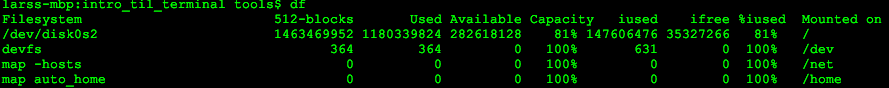
\includegraphics[scale=0.55]{images/df_std.png}
\subsection{-h - Menneskligt læsligt}
Som kan ses på outputtet i billedet her over, er outputet ikke videre forståeligt, for ikke teknisk folk. Men \textit{df} har et flag som er \textit{-h}, som giver et bedere og mere læsbar output og kaldes således \textit{df -h}.\\
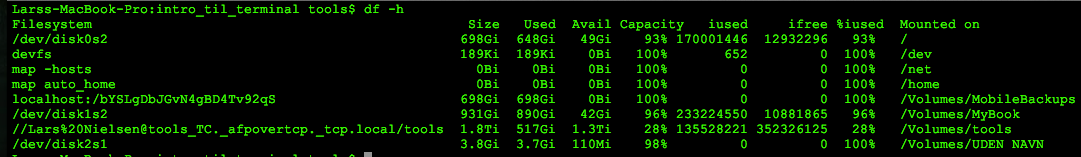
\includegraphics[scale=0.45]{images/df_h.png} 
